\newpage
\section{Experiment}
\label{sec:exp}


\subsection{Corpus}
We conduct our experiments on three types of corpus.
\begin{itemize}
\item  The first corpus is the Stanford sentiment treebank released by Socher et. al. (2013). It is based on the dataset introduced by Pang and Lee (2005) and consists of 11,855 single sentences extracted from movie reviews on \url{http://www.rottentomatoes.com/}. It was parsed with the Stanford parser (Klein and Mannning, 2003) and includes a total of 215,154 unique phrases from those parse trees, each annotated by 3 human judges. To the best of our knowledge, it is the only public available corpus upon which a RNTN sentiment model can be trained right now. We refer to this corpus by \textit{Sentiment Treebank} in the reset of paper. 

\item  The second corpus is movie reviews on Twitter. We have 364 tweets extracted from two specialized review accounts (@FilmReviewIn140, @MovieTwoosh). Such reviews are mostly well formatted, usually consist of several sentences. The author rated each movie with A to F grades and the label the sentiment of the tweet base on the grade. Tweets with a grade no worse than B are labeled positive otherwise negative.  We refer to this corpus by \textit{moive} in the reset of paper. 

\item The third corpus is general tweet message. It is taken from SemEval-2013: Sentiment Analysis in Twitter Task B\footnote{\url{http://www.cs.york.ac.uk/semeval-2013/task2/index.php?id=data}}. In their release, each of the tweet messages has been manually labeled as positive, negative, or neutral. Out of all the 5,750 messages, 2,042 are positive, 855 are negative and 2853 are neutral.  We refer to this corpus by \textit{SemEval} in the reset of paper. 
\end{itemize}

\subsection{Single Sentence Sentiment}
We firstly evaluate both models using \textit{Sentiment Treebank}, The same training/testing splits as in the original paper\cite{Socher:2013} is used. 

\begin{table}[H]
  \begin{center}
    \begin{tabular}{cccc}\hline
      \multirow{2}{*}{Model} 
      & \multicolumn{3}{c}{Accuracy} \\\cline{2-4}
    & positive & negative & overall \\ \hline
    RNTN  & 80.83      &   87.91   &  84.27      \\ 
    SVM$_S$  & 74.15      &  73.79    &    73.97     \\ 
    SVM$_L$  & 75.90      & 73.90         &   74.90      \\ \hline
    \end{tabular}
    \end{center}
    \caption{\label{exp_1} Binary decision}
\end{table}

In SVM$_S$, we use a smaller dictionary (1635 words) in which words appear more than 10 times are used. In SVM$_L$, we build a larger dictionary (3504 words) with the bar lowered to 5 times. 

As we can see from Table \ref{exp_1}, the performance of RNTN model is significantly better than SVM models. This is consistent with the result of the original paper\cite{Socher:2013}. The huge boost comes from the fact that the structure of the sentence is utilized in the RNTN model. It might seems to be an unfair comparison as more information is needed (the sentiment of each parse of the sentence) in training the RNTN model. 
However, even if we train the SVM model with sentiment label of each parse as well, the result won't improve much as what SVM sees is just a subset of the original bag.  


\subsection{Multiple Sentences Sentiment}
We then evaluate how to combine the sentiment multiple sentences. This is not an issue of SVM because only a larger bag is needed. However, RNTN relies on the structural of single sentence so we need to combine the sentiment from multiple sentences within a single tweet. Here, we train the model on \textit{Sentiment Treebank} and test it on \textit{movie} corpus. 

As for the RNTN model, we evaluate two ways to combine the sentiment of the whole tweet (multiple sentences). The first is to make hard (binary) decision on single sentence ( either positive or negative) and sentiment of the tweet is decided by majority vote. Soft information (probability) is only used to break a tie. The second way fully relis on soft (probability) information. For each sentence, we generate a 5-element vector for the probability of the having the corresponding sentiment (very negative, negative, neutral, positive, very positive). We add the vector for all the sentences together and make final decision based on the combined vector. 
\begin{table}[H]
  \begin{center}
    \begin{tabular}{cccc}\hline
      \multirow{2}{*}{Model} 
      & \multicolumn{3}{c}{Accuracy(\%)} \\\cline{2-4}
    & positive & negative & overall \\ \hline
    RNTN$_{hard}$  & 70.08 	    &  81.54       &  74.18     \\
    RNTN$_{soft}$  & 78.21     &   80.0	    &   78.85    \\ 
    SVM           & 73.50     &   66.92     &   71.15      \\\hline 
    \end{tabular}
    \end{center}
    \caption{\label{exp2_1} Binary decision}
\end{table}

From Table \ref{exp2_1}, we can see that both RNTN models perform better than SVM. For the two RNTN models, 
 hard decision model has worse performance than soft decision in positive sentiment but slightly better on negative sentiment. This indicates that RNTN model tend to label a sentence as negative. Soft combining outperforms hard combining by more than 4\% in the overall result. This is reasonable because more information is available in soft decision combining. Based on the above result, we use soft mode in the following experiments. 

%\subsection{Effect of Preprocessing}
%We also evaluates how much preprocessing contributed to our final performance. In this experiment, we still use the model trained on \textit{Sentiment Treebank} but tested on \textit{movieB} corpus, which contains noisy common twitter message collected by searching movie names. We evaluated both models with and without preprocessing the original corpus. 
%
%\begin{table}[H]
%  \begin{center}
%    \begin{tabular}{ccc}\hline
%      \multirow{2}{*}{Model} 
%      & \multicolumn{2}{c}{Overall Accuracy(\%)} \\\cline{2-3}
%    & with pre-processing & w/o pre-processing \\ \hline
%    RNTN  &          &     	       \\ 
%    SVM1  & ~        &              \\ 
%    SVM2  & ~        &              \\ \hline
%    \end{tabular}
%    \end{center}
%    \caption{\label{exp5_3} Effect of preprocessing}
%\end{table}
%
%Comparing both table, we can see that preprocessing indeed helped in improving the performance.  

\subsection{General topic Tweet}
We conducted three sets of experiment over the general topic twitter corpus \textit{SemEval}. 
\begin{itemize}
\item Exp 1: Training on 90\% of \textit{SemEval} and testing on the rest 10\%. 

This is the classic experiment setup. However, as we don't have annotated sentiment parse tree  (the sentiment of each node of the parse tree, which is required to train the RNTN model), a RNTN model based on \textit{SemEval} can not be trained. Thus, we evaluate different features of SVM model in this experiment. 

\begin{table}[H]
  \begin{center}
    \begin{tabular}{llc}\hline
     \multicolumn{2}{c}{Feature} & Accuracy (\%)     \\\hline
     \multirow{3}{*}{Unigram}    & Binary feature  &  78.84  \\ 
                                 & Frequency       &  78.64  \\ 
                                 & Tf-idf          &  78.22 \\
     \multicolumn{2}{l}{Bigram}                    &  70.41 \\    
     \multicolumn{2}{l}{Unigram-url-num}           &  \textbf{79.32} \\
     \multicolumn{2}{l}{Unigram-elongated}         &  79.01 \\
     \multicolumn{2}{l}{Unigram-url-num-elongated} &  79.19 \\
     \multicolumn{2}{l}{Unigram-neg}               &  78.77 \\
     \multicolumn{2}{l}{Unigram-neg-url-num}       &  78.19 \\
     \multicolumn{2}{l}{Unigram-neg-enlongated}    &  78.34 \\
     \multicolumn{2}{l}{Unigram-neg-url-num-enlongated}  &  77.95 \\\hline      
    \end{tabular}
    \end{center}
    \caption{\label{exp5_1} Experiment 1}
\end{table}

Begin. \vspace{5cm} Discuss the result here. 


\item Exp 2: Training on \textit{Sentiment Treebank} and testing on \textit{SemEval}. \\ 
In this experiment, we apply the model trained on \textit{Sentiment Treebank} on the general topic twitter message. It may sounds wired but as we mentioned earlier, \textit{Sentiment Treebank} is the only corpus upon which we can train RNTN model. To be fair, we train a SVM model in the same way and compare the performance of the two in both binary-decision and ternary-decision task. 
\begin{table}[H]
  \begin{center}
    \begin{tabular}{cccc}\hline
      \multirow{2}{*}{Model} 
      & \multicolumn{3}{c}{Accuracy(\%)} \\\cline{2-4}
    & positive & negative & overall \\ \hline
    RNTN  & 69.83     &   70.17	    &   69.93    \\ 
    SVM   & 67.14     &   60.91     &   65.30      \\ \hline
    \end{tabular}
    \end{center}
    \caption{\label{exp5_2_1} Experiment 2.1}
\end{table}

\begin{table}[H]
  \begin{center}
    \begin{tabular}{ccccc}\hline
      \multirow{2}{*}{Model} 
      & \multicolumn{4}{c}{Accuracy(\%)} \\\cline{2-5}
    & positive & negative & neutral & overall \\ \hline
    RNTN  & 48.12    &   43.17  	   &   49.40       & 48.02    \\ 
    SVM   & 52.52    &   23.86     &   44.69       & 37.14    \\ \hline
    \end{tabular}
    \end{center}
    \caption{\label{exp5_2_2} Experiment 2.2}
\end{table}

From Table \ref{exp5_2_1} and Table \ref{exp5_2_2}, we can see that RNTN out perform SVM in both binary decision and ternary decision. However, the performance is worse than the result from Table \ref{exp5_1}. 

The huge decrease in SVM model resulted from the difference of the two corpus. 
Clearly, twitter specific feature helps SVM model a lot but such feature is not available in the \textit{Sentiment Treebank}. 

Another interesting comparison is the performance of RNTN in Table \ref{exp_1} and Table \ref{exp5_2_2}. Like statistical parser, RNTN model is also quite specific to the genre of the training corpus. To make the problem worse, the Stanford parse doesn't work quite well on twitter message due to the noisy nature of it. 

\item Exp 3: Domain adaptation of RNTN\\
In this experiment, we explore domain adaptation of RNTN sentiment model. This is an interesting experiment as gathering fully annotated training data on twitter message is expensive and labor intensive. We have fully annotated corpus in \textit{Sentiment Treebank} but \textit{SemEval} is only been labeled positive, neutral or negative. In this experiment, we first train the model on \textit{Sentiment Treebank}, then use the above model to label the training set of \textit{SemEval} in sentiment treebank format. We retrain the model with both \textit{Sentiment Treebank} and the labeled  training set of \textit{SemEval}. In the end, we test the new model on the test set of \textit{SemEval}.


%\begin{table}[H]
%  \begin{center}
%    \begin{tabular}{cccc}\hline
%      \multirow{2}{*}{Model} 
%      & \multicolumn{3}{c}{Accuracy(\%)} \\\cline{2-4}
%    & positive & negative & overall \\ \hline
%    RNTN  &          &     	   &      \\ 
%    SVM1  & ~        &          &         \\ 
%    SVM2  & ~        &          &         \\ \hline
%    \end{tabular}
%    \end{center}
%    \caption{\label{exp5_3_1} Experiment 3.1}
%\end{table}


%\begin{table}[H]
%  \begin{center}
%    \begin{tabular}{ccccc}\hline
%      \multirow{2}{*}{Model} 
%      & \multicolumn{4}{c}{Accuracy(\%)} \\\cline{2-5}
%    & positive & negative & neutral & overall \\ \hline
%    Binary  & ~        &   ~	   &   --         &    \\ 
%    Ternary  & ~        &          &             &   \\ \hline
%    \end{tabular}
%    \end{center}
%    \caption{\label{exp5_3} Experiment 3}
%\end{table}

\begin{figure}[H]
\begin{center}
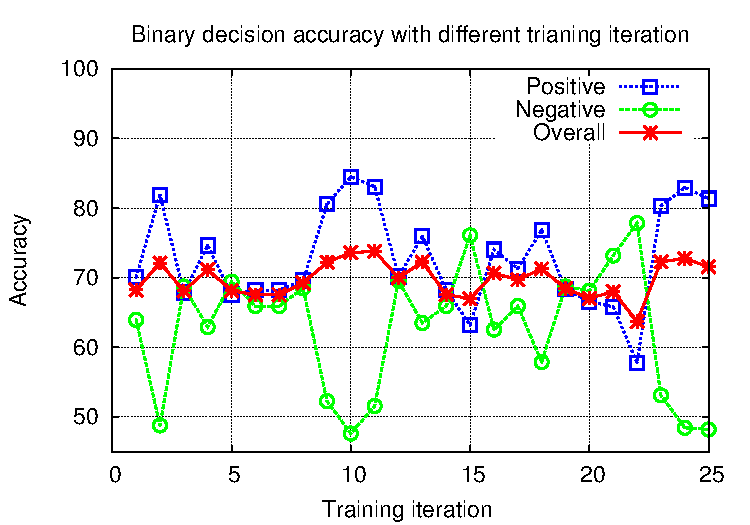
\includegraphics[width = 0.5\textwidth]{pic/model_2b.pdf}
\caption{Binary decision }
\end{center}
\end{figure}

\begin{figure}[H]
\begin{center}
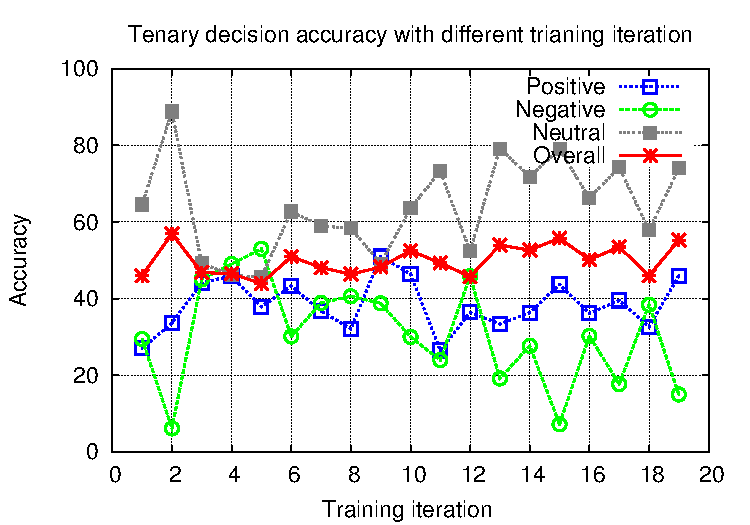
\includegraphics[width = 0.5\textwidth]{pic/model_3c.pdf}
\caption{Ternary decision }
\end{center}
\end{figure}

We train the model with different iterations and evaluate all the models. As we can see from the above two figures, the result fluctuates a lot. Unfortunately, we don't see significant improvement in performance with domain adaptation.  




\end{itemize}







